\documentclass[conf]{new-aiaa}
%\documentclass[journal]{new-aiaa} for journal papers
\usepackage[utf8]{inputenc}

\usepackage{graphicx}
\usepackage{amsmath}
\usepackage[version=4]{mhchem}
\usepackage{siunitx}
\usepackage{longtable,tabularx}
\usepackage{footnote}
\usepackage{mhchem}
\usepackage{physics}
\usepackage{array,makecell,booktabs}
\newcolumntype{M}[1]{>{\centering\arraybackslash}m{#1}}
\usepackage[super]{nth}
\makesavenoteenv{tabular}
\setlength\LTleft{0pt} 

\graphicspath{{figures/}}

\title{Preparation of Papers for AIAA Technical Conferences}

\author{First A. Author\footnote{Insert Job Title, Department Name, Address/Mail Stop, and AIAA Member Grade (if any) for first author.} and Second B. Author Jr.\footnote{Insert Job Title, Department Name, Address/Mail Stop, and AIAA Member Grade (if any) for second author.}}
\affil{Business or Academic Affiliation 1, City, State, Zip Code}
\author{Third C. Author\footnote{Insert Job Title, Department Name, Address/Mail Stop, and AIAA Member Grade (if any) for third author.}}
\affil{Business or Academic Affiliation 2, City, Province, Zip Code, Country}
\author{Fourth D. Author\footnote{Insert Job Title, Department Name, Address/Mail Stop, and AIAA Member Grade (if any) for fourth author (etc.).}}
\affil{Business or Academic Affiliation 2, City, State, Zip Code}

\begin{document}

\maketitle

\begin{abstract}
These instructions give you guidelines for preparing papers for AIAA Technical Papers using \LaTeX{}. Define all symbols used in the abstract. Do not cite references in the abstract. The footnote on the first page should list the Job Title and AIAA Member Grade for each author, if known Authors do not have to be AIAA members.
\end{abstract}

\section{intro/motivation}

\section{Description of Recovery Strategies}
Although only two vehicles with recoverable stages have been operated, a wide variety of first stage recovery strategies have been proposed. This section seeks to develop a systematic classification of recovery strategies, which will be useful in comparing their relative merits.

First stage recovery strategies can be characterized by three high-level choices:
\begin{enumerate}
	\item \textit{Portion of stage recovered} - Some strategies recover the entire first stage, while others propose to only recover a portion containing the higher-value components (e.g. main engines).
	\item \textit{Deceleration and maneuvering method} - The first stage must have some means to control and slow its re-entry trajectory. The deceleration and maneuvering methods can be grouped into three categories: propulsive designs which use the main engines to maneuver and land vertically; winged designs which use aerodynamic surfaces to maneuver and land horizontally; and design which decelerate using parachutes. Note that these are not absolute distinctions: current propulsive-landing designs use small aerodynamic control surfaces, and some proposed winged designs have auxiliary propulsion to increase their range.
	\item \textit{Recovery location} - The stage may be recovered downrange, or may fly itself back for recovery at the launch site. Most downrange recovery strategies land on a boat or in the ocean, although some call for the recovered components to be caught by an aircraft in midair \cite{Ragab2015}.
\end{enumerate}

Figure \ref{fig:recov_strat_diagram} illustrates the concept of operations for various strategies formed from the above choices. Strategies which have been carried out or proposed are listed in Table \ref{tab:vehicles}, and along the bottom of Figure \ref{fig:recov_strat_diagram}.

\begin{figure}[hbt!]
	\centering
	\includegraphics[width=1\textwidth]{figures/recov_strat_diagram}
	\label{fig:recov_strat_diagram}
	\caption{Recovery strategies TODO better graphics}
\end{figure}

\begin{table}
	\caption{\label{tab:vehicles} Some launch vehicles with reusable first stages. (* denotes boosters used in parallel staging)}
	\centering
	\begin{tabular}{p{4cm} l p{2cm}  p{2cm} p{2cm}}
		\hline
		Vehicle & Status & Portion of booster recovered & Deccel \& Manuever method & Recovery location \\
		\hline
		\hline
		Falcon 9 & Operational & Full & Propulsive & Launch site or downrange \\
		\hline
		Space Shuttle* & Retired & Full & Parachute & Downrange \\
		\hline
		New Glenn & Proposed & Full & Propulsive & Downrange \\
		Adeline (Ariane 6) & Proposed & Partial & Wing & Launch site \\
		SMART (Vulcan) \cite{Ragab2015} & Proposed & Partial & Parachute & Downrange midair \\
		\hline
		Ares I \cite{Ares2009} & Canceled & Full & Parachute & Downrange \\
		Reusable Booster System (RBS) \cite{NAP13534} & Canceled & Full & Propulsive \& Wing & Launch site\\
		NASA Liquid Fly-Back Booster (LFBB)* \cite{Healy1998} & Canceled & Full & Propulsive \& Wing & Launch site\\
		DRL Liquid Fly-Back Booster (LFBB)* \cite{Sippel2003} & Canceled & Full & Propulsive \& Wing & Launch site\\
		\hline
	\end{tabular}
\end{table}

Despite their wide variety, all these strategies face the same fundamental tradeoff between performance and cost. On the performance side, all recovery strategies require the first stage to carry extra mass during ascent, reducing the payload which can be lifted to orbit. However, recovering and reusing some of the first stage has the potential to reduce launch costs by eliminating the need to re-build expensive hardware\footnote{A reduction in cost is by no means guaranteed. As the Space Shuttle program demonstrated, excessive refurbishment and operations costs can make a reusable system more expensive than expendable alternatives.}. We should expect that recovery strategies will differ in their performance penalty and potential for cost reduction. The fundamental question is which, if any, of the recovery strategies can offer a small enough payload reduction and a large enough cost reduction to be worthwhile?

To make this question more concrete, this paper defines two figures of merit for recovery strategies: the payload factor $r_p$ and the cost factor $r_c$. These factors compare the payload capacity and cost of a vehicle with a reusable first stage to an equivalent\footnote{The `equivalent' expendable vehicle uses the same propulsion and structural technologies, and has the same gross liftoff mass $m_{0,1}$} vehicle with an expendable first stage. The payload factor is the payload capacity of the partially reusable vehicle divided by the payload capacity of the equivalent expendable vehicle. The cost factor is the average flight cost of the reusable first stage divided by the average flight cost of an expendable first stage.

When comparing recovery strategies, we can largely neglect their internal complexities and consider each strategy to be represented by a tuple $\mathcal{R}: \{r_p, r_c\}$. We seek recovery strategies with high payload factor ($r_p \rightarrow 1$) and low cost factor ($r_c \rightarrow 0$).

The following two sections attempt to provide quantitative, first-principles tools to estimate $r_p$ and $r_c$. The payload factor can be easily estimated with a fair degree of accuacy, but cost modeling involves more guesswork. The TODO nth section examines the trade-offs between different strategies. Because the willingness of a launch provider to trade payload for cost is uncertain, this comparison is framed to yield a set of recovery strategies which is Pareto-optimal in $(r_p, r_c)$.




\section{Performance Model}
TODO
This section provides a general, first-principles framework for estimating the payload reduction factor $r_p$ of a recovery strategy. The fundamental cause of payload reduction is that a recoverable stage must carry extra mass, as recovery hardware or propellant reserved for recovery maneuvers. This extra mass reduces the fraction of the stage's mass which is expelled during ascent. To still deliver the required $\Delta v$ to the payload, the payload mass fraction must then be reduced.

\subsection{Payload factor and first stage unavailable mass}
This subsection establishes a relationship between the payload factor $r_p$ and the extra mass carried on the first stage for recovery.
The reduction in payload can be seen from the Tsiolkovsky rocket equation. For a two-stage, sequentially stage rocket, the equation is \cite{Wiesel2010}:

\begin{equation}
\Delta v_* =  \sum_{i=1}^{2} - c_i \ln\left( \epsilon_i + (1 - \epsilon_i) \pi_i \right)
\end{equation} 

$\Delta v_*$ is the `mission $\Delta v$' required to lift the payload to its desired orbit. $c_i$ is the effective exhaust velocity ($c = I_{sp} g_0$) of stage $i$, averaged over the ambient pressures at which the stage operates. The log-mass term is written in terms of the dimensionless parameters $\epsilon_i$ and $\pi_i$. $\epsilon_i$ is the inert mass fraction of stage $i$; it depends only on the design of the stage.

\begin{equation}
\epsilon_i = \frac{m_{s,i}}{m_{s,i} + m_{p,i}}
\end{equation}

$\pi_i$ is the mass of the stage's payload (including all higher stages) divided by the gross mass at stage ignition:

\begin{equation}
\pi_1 = \frac{m_{0,2}}{m_{0,1}}, \quad \pi_2 = \frac{m_*}{m_{0,2}}
\end{equation}

The overall payload ratio of the launch vehicle, $\pi_*$ is the product of the stage payload ratios:

\begin{equation}
\label{eq:pi_star}
\pi_* = \frac{m_*}{m_{0,1}} = \pi_1 \pi_2
\end{equation} 

Modifying the rocket for first stage recovery effectively increases the inert mass fraction of the first stage to some new value $\epsilon_1'$. I will call $\epsilon_1'$ the `unavailable mass fraction', as it is the fraction of the first stage's mass which is unavailable for expulsion to propel the ascent. It includes the mass of the first stage structure ($m_{s,1}$) , the mass of recovery hardware ($m_{rh,1}$), and the mass of propellant reserved for recovery maneuvers ($m_{pr,1}$). The unavailable mass fraction can also be thought of as the first stage mass at stage separation divided by the first stage mass at liftoff.

\begin{equation}
\label{eq:epsilon_1_prime}
\epsilon_1' = \frac{m_{s,1} + m_{rh,1} + m_{pr,1}}{m_{s,1} + m_{rh,1} + m_{p,1}}
\end{equation}

Then, the rocket equation for ascent is
\begin{equation}
\label{eq:recov_rocket}
\Delta v_* =  - c_1 \ln\left( \epsilon_1' + (1 - \epsilon_1') \pi_1 \right) - c_2 \ln\left( \epsilon_2 + (1 - \epsilon_2) \pi_2 \right)
\end{equation}

Our goal is to use Equation \ref{eq:recov_rocket} to determine how changes to $\epsilon_1'$ affect $\pi_*$. To do this, we need to introduce a few additional constraints. First, we assume that the stage 2 / stage 1 mass ratio has a some value $y$.

\begin{equation}
y = \frac{m_{s,2} + m_{p,2}}{m_{s,1} + m_{rh,1} + m_{p,1}}
\end{equation}

For current U.S. 2-stage launch vehicles, $y$ is 0.076 to 0.265 (see Table \ref{tab:tech_and_payload}). It can be shown that

\begin{equation}
\label{eq:ypi}
\pi_2 = (y + 1) - \frac{y}{\pi_1}
\end{equation}

Second, we define a `technology choice', $\mathcal{T}$, which influences the mass ratios and exhaust velocities. This choice encompasses technological factors such as the propellant (e.g. \ce{O2(l)}/kerosene vs. \ce{O2(l)}/\ce{H2(l)}), the tank construction technology (e.g. aluminum alloy vs. composite), and the engine cycle (e.g. gas generator vs. staged combustion). For the purposes of this model, the technology choice is fully described by the tuple $\mathcal{T} : \{ c_1, c_2, E_1, E_2 \}$, where $E$ is the technological lower limit on the structural mass fraction of an expendable stage. For expendable stages, $\epsilon_i = E_i$. For recoverable stages, $\epsilon_1' > E_1$. Table \ref{tab:tech_and_payload} lists example technology choices and payload ratios for some U.S. launch vehicles.

\begin{table}
	\caption{\label{tab:tech_and_payload} Technology choices and payload ratios for U.S. Evolved "Expendable" Launch Vehicles. ($c_1$ is mean of vacuum and sea level values. GTO at \ang{27} inclination, \SI{185 x 35788}{\kilo\meter}.)}
	\centering
	\begin{tabular}{p{3cm} M{2.5cm} M{2.5cm} c c c}
		Vehicle & \multicolumn{2}{c}{Technology choice $\mathcal{T}$} & Stage mass ratio $y$ & \multicolumn{2}{c}{Payload ratio $\pi_*$} \\
		 & \nth{1} stage & \nth{2} stage & & LEO & GTO \\
		 \hline
		 \hline
		 
		 Delta IV Medium \newline \cite{Slazer2017, slr:delta_iv}
		 & $c_1/g_0=\SI{386}{\second}$ \newline $E_1=0.121$ \newline \ce{H2(l)}/\ce{O2(l)} \newline Gas gen. cycle \newline \ce{Al} alloy tanks
		 & $c_2/g_0=\SI{462}{\second}$ \newline $E_2=0.120$ \newline \ce{H2(l)}/\ce{O2(l)} \newline Expander cycle \newline \ce{Al} alloy tanks
		 & 0.100 & 0.034 & 0.016 \\
		 
		 \hline
		 
		 Atlas V 401 \newline \cite{atlas_v_user_guide, slr:atlas_v}
		 & $c_1/g_0=\SI{325}{\second}$ \newline $E_1=0.069$ \newline kerosene/\ce{O2(l)} \newline Staged cb. cycle \newline \ce{Al} alloy tanks
		 & $c_2/g_0=\SI{450}{\second}$ \newline $E_2=0.100$ \newline \ce{H2(l)}/\ce{O2(l)} \newline Expander cycle \newline Steel tanks
		 & 0.076 & 0.029 & 0.014 \\
		 
		 \hline
		 
		 Falcon 9 Block 3 \newline (expendable $\pi_*$) \cite{slr:falcon_9}
		 & $c_1/g_0=\SI{297}{\second}$ \newline $E_1 \leq 0.062$ \newline kerosene/\ce{O2(l)} \newline Gas gen. cycle \newline \ce{Al-Li} alloy tanks
		 & $c_2/g_0=\SI{350}{\second}$ \newline $E_2=0.039$ \newline kerosene/\ce{O2(l)} \newline Gas gen. cycle \newline \ce{Al-Li} alloy tanks
		 & 0.265 & 0.030 & 0.011 \\
		 
		 \hline
	\end{tabular}
\end{table}

If we know $\Delta v_*$ (set by the mission), the technology choice $\mathcal{T}$, and the stage mass ratio $y$, we can find $\pi_*(\epsilon_1')$ from Equations \ref{eq:pi_star}, \ref{eq:recov_rocket}, and \ref{eq:ypi}. This relation is explored in Figure \ref{fig:stage_mass_ratio}, which plots $\pi_*$ versus $y$ for various $\mathcal{T}$ and $\epsilon_1'$. Each subplot assumes a different technology choice; the technology choice values are taken from the U.S. EELV fleet (left: Delta IV, center: Atlas V, right: Falcon 9). The black curve shows $\pi_*$ versus $y$ for a vehicle with $\epsilon_1=E_1$. The solid black lines mark the actual stage mass ratio and (expendable mode) payload ratio for the vehicle on which the technology choice is based. If the model accurately describes the vehicle's payload capacity, the black curve should pass through the intersection of the black lines. In fact, the model slightly over-predicts $\pi_*$ (perhaps because it neglects the mass of the payload fairing).  
Each colored curve shows $\pi_*$ versus $y$ for a different hypothetical values of $\epsilon_1'$. On each curve, the maximum payload point is marked with a dot.

We can notice a few to-be-expected trends. First, the payload capacity decreases as the first stage unavailable mass increases. Second, for almost all combinations of $y$ and $\epsilon_1'$, the \ce{H2(l)} fuel technology choice (`Delta IV'-like, left) has a higher payload ratio than kerosene fuel (`Falcon 9'-like, right). The higher $I_{sp}$ of \ce{H2(l)} more than compensates for the heavier tanks required by its low density.

The variation of the payload-optimal $y$ with $\epsilon_1'$ is more interesting. Intuitively, we might expect that as $\epsilon_1'$ increases, the first stage becomes `less efficient', so $y$ should be increased to shift more of the mission $\Delta v$ to the higher-performing second stage. This is true for the `Falcon 9'-like technology choice (right subplot), and also appears in McKinney's first stage recovery study \cite{McKinney1986}. However, for the other two technology examples, the payload-optimal $y$ is almost constant as $\epsilon_1'$ increases.

It is also interesting to compare the actual $y$ values to the (predicted) payload-optimal $y$. The Atlas V stage mass ratio is far below the optimal value - for historical reasons, Atlas V uses the Centaur upper stage, which was originally designed for a smaller launch vehicle. In contrast, Falcon 9's second stage is bigger-than-optimal for expendable use ($\epsilon_1=0.06$), but is near the optimal $y$ if recovery provisions increase $\epsilon_1'$ to $~0.13$. The predicted payload capacity at $\epsilon_1' \approx 0.13$ matches the actual payload capacity of Falcon 9 with downrange recovery of the first stage (right subplot, black dashed line).

\begin{figure}[hbt!]
	\centering
	\includegraphics[width=\textwidth]{../stage_mass_ratio}
	\caption{\label{fig:stage_mass_ratio} Effect of first stage unavailable mass fraction $\epsilon_1'$ and stage mass ratio $y$ on payload capacity.}
\end{figure}

Next, we want to compare the payload capacity of the recoverable rocket to that of an equivalent expendable rocket to find the payload factor $r_p$. First, we will make our definition of `equivalent expendable rocket' more rigorous: the `equivalent' rocket uses the same technology choice, the same stage mass ratio, and has the same gross liftoff mass. We also assume that the mission $\Delta v_*$ is the same for both rockets \footnote{We might expect this assumption to be incorrect if the recovery strategy changes the $\Delta v$ losses during ascent (e.g. increased drag due to wings). However, an analysis by DRL finds that ``The impact of the different RLV-types [reusable launch vehicle] on the ascent flight profile is found small and, similar to the ELV [expendable launch vehicle] ascent flight performance losses, these are more dependent on the particular configuration with its T/W [thrust to weight] ratio than on the landing and return modes.'' \cite{Stappert2017}.}

\begin{equation}
\mathcal{T}^{\mathrm{expend}} = \mathcal{T}^{\mathrm{recov}}, \quad y^{\mathrm{expend}} = y^{\mathrm{recov}}, \quad m_{0,1}^{\mathrm{expend}} = m_{0,1}^{\mathrm{recov}}, \quad \Delta v_*^{\mathrm{expend}} = \Delta v_*^{\mathrm{recov}}
\end{equation}

Finally, the payload factor is

\begin{equation}
r_p = \frac{m_*^{\mathrm{recov}}}{m_*^{\mathrm{expend}}} = \frac{\pi_*^{\mathrm{recov}}}{\pi_*^{\mathrm{expend}}}
\end{equation}

The relation of $r_p$ to $\epsilon_1'$ is shown in Figure \ref{fig:payload} for two typical launch missions (Low Earth Orbit $\Delta v_* = \SI{9.5}{\kilo\meter\per\second}$, blue; and Geostationary Transfer Orbit $\Delta v_* = \SI{12.0}{\kilo\meter\per\second}$, orange) and two technology choices (`Delta IV'-like with \ce{H2(l)} fuel, left subplots; and `Falcon 9'-like with kerosene fuel, right subplots). On the kerosene plot, the actual $r_p$ values for Falcon 9 Block 3 \cite{slr:falcon_9} are indicated by dashed horizontal lines. As expected, the payload capacity declines with increasing first stage unavailable mass. Also, note that the decline is more severe for higher $\Delta v_*$ missions. Thus, a particular recovery strategy (with some $\epsilon_1'$) will have a smaller payload factor for GTO missions than for LEO missions ($r_p^{\mathrm{LEO}} > r_p^\mathrm{GTO}$). Higher $\Delta v_*$ missions put a bigger penalty on first stage recovery. Also notice that the payload reduction factors are similar for both technology choices - neither is inherently better suited for recovery. In either case, increasing $\epsilon_1'$ from $E_1$ to 0.23 halves the payload capacity to GTO.

\begin{figure}[hbt!]
	\centering
	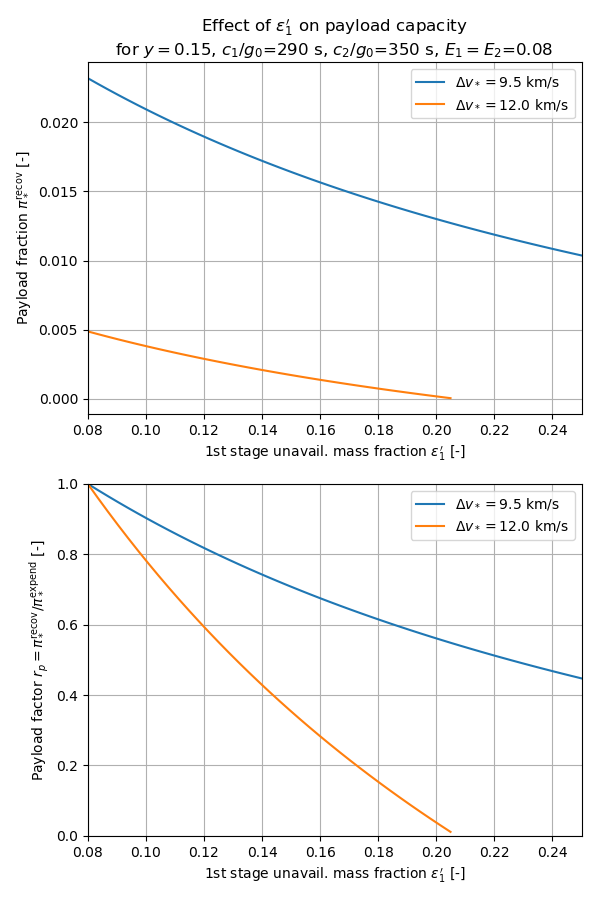
\includegraphics[width=\textwidth]{../payload}
	\label{fig:payload}
	\caption{Impact of first stage unavailable mass fraction $\epsilon_1'$ on payload capability. Note that the payload factor $r_p$ declines with increasing unavailable mass, and the decline is more severe for higher $\Delta v_*$ missions.}
\end{figure}


\subsection{Determining the unavailable mass from recovery hardware and maneuvers}
This subsection provides techniques for estimating the unavailable mass fraction $\epsilon_1'$ from the hardware and maneuvers needed to recover the stage. The mathematics are best approached by imagining that we start with an expendable first stage, and then modify the stage so that it can be recovered (also, this is an actual development strategy, e.g. Falcon 9 and SMART). Suppose our baseline expendable stage has a dry mass $m_{s,1}$ and a can carry a propellant load $m_{p,1}$ \footnote{Assume the propellant load does not change when the stage is modified for recovery}. The baseline stage contains some high-value hardware which we wish to recover, with mass $m_{hv}$. Let $z_m$ be the fraction of the baseline stage hardware which we wish to recover:

\begin{equation}
z_m \equiv \frac{m_{hv,1}}{m_{s,1}}
\end{equation}

In full recovery strategies, we wish to recover the entire first stage, so $m_{hv,1} = m_{s,1}$ and $z_m=1$. For partial recovery strategies, we only wish to recover part of the first stage (e.g. the engines), so $m_{hv,1} < m_{s,1}$ and $z_m \in (0, 1)$. Some unwanted hardware with mass $m_{s,1}(1 - z_m)$ is discarded shortly after stage separation.

To enable recovery, we will likely have to add some hardware to the stage, with mass $m_{rh,1}$. This includes, for example, the mass of wings, control surfaces, heat shields and landing gear added to the stage. It also includes any increase in mass (e.g. of the structure or engines) incurred by design requirements for re-usability or recovery loads. Let `recovery vehicle' denote the set of first stage components which are recovered at the end of the mission. For full recovery, the recovery vehicle is the entire first stage; for partial recovery it is perhaps a small pod containing the engines. The recovery vehicle has a touchdown (dry) mass of $m_{rh,1} + m_{hv,1}$.

Next, consider how efficiently we are able to make use of mass on the recovery vehicle. Let us define $a$ to be the fraction of the recovery vehicle dry mass which is added recovery hardware.

\begin{equation}
a \equiv \frac{m_{rh,1}}{m_{rh,1} + m_{hv,1}}
\end{equation}

A fraction $1-a$ of the recovery vehicle mass is the mass of the high value components which we set out to recover. By definition $a \in [0, 1]$. The extreme $a=0$ represents the (rather miraculous) situation in which we could recover the high value hardware in its bare expendable configuration, without any additional recovery equipment. The extreme $a \rightarrow 1$ represents the situation in which our recovery vehicle construction is very poor, and many tons of wings, parachutes, etc. are needed to recover a few kilograms of high-value hardware.

The recovery vehicle may need some propellant to perform maneuvers during the recovery process. Let the mass of this propellant be $m_{pr,1}$. The recovery propellant mass is related to the recovery vehicle dry mass by:

\begin{equation}
m_{pr,1} = (m_{rh,1} + m_{hv,1}) \left( e^P - 1 \right)
\end{equation}

The exponent $P$ depends on the type of maneuvers performed. If the recovery maneuvers use rocket propulsion, then $P$ is found from the Tsiolkovsky equation:

\begin{equation}
\label{eq:rocket_p}
P = \frac{\Delta v_r}{c_1}
\end{equation}

where $\Delta v_r$ is the $\Delta v$ of the recovery maneuvers. If instead the recovery vehicle flies back and uses air-breathing propulsion to maintain steady level flight, then $P$ is found from the Berguet range equation:

\begin{equation}
\label{eq:berguet_p}
P =  \frac{R_{\mathrm{cruise}}}{v_{\mathrm{cruise}} (L/D) I_{sp}^{ab}}
\end{equation}

where $R_{\mathrm{cruise}}$ is the cruise range, $v_{\mathrm{cruise}}$ is the cruise speed, $(L/D)$ is the cruise lift to drag ratio and $I_{sp}^{ab}$ is the specific impulse of the air breathing engine. If no (mass-expelling) propulsion is used during recovery, $P = 0$ and $m_{pr,1} = 0$.

To summarize the above discussion, Figure \ref{fig:recov_mass_flow} tracks the mass of the first stage through the mission. At liftoff, the first stage has a hardware mass $m_{s,1} + m_{rh,1}$ and carries a propellant mass $m_{p,1}$. During ascent, the first stage burns a mass $m_{p,1} - m_{pr,1}$ of propellant. Shortly after stage separation, a mass $m_{s,1} - m_{hv,1}$ of unwanted hardware may be discarded (if the recovery strategy is partial). The remainder of the stage  (recovery vehicle) then maneuvers to the recovery location. If this maneuver uses propulsion, the remaining propellant mass $m_{pr,1}$ is burned during the maneuver. Finally, at the time of recovery, the remaining mass of hardware is $m_{rh,1} + m_{hv,1}$ and no propellant is left \footnote{Propellant residuals/reserves are counted in $m_{rh,1}$}.

\begin{figure}[hbt!]
	\centering
	\includegraphics[width=0.8\textwidth]{figures/recov_mass_flow}
	\caption{\label{fig:recov_mass_flow} Changes in mass of the first stage/recovery vehicle during the mission.}
\end{figure}

Now we are equipped to find an expression for the first stage unavailable mass fraction $\epsilon_1'$. Start from Equation \ref{eq:epsilon_1_prime} and divide the numerator and denominator by $m_{s,1}$.

\begin{equation}
\epsilon_1' = \frac{1 + \frac{m_{rh,1}}{m_{s,1}} + \frac{m_{pr,1}}{m_{s,1}} }{1 + \frac{m_{rh,1}}{m_{s,1}} + \frac{m_{p,1}}{m_{s,1}} }
\end{equation}

From the above definitions, it can be shown that:

\begin{equation}
\frac{m_{rh,1}}{m_{s,1}} = \frac{a z_m}{1 - a}
\end{equation}

\begin{equation}
\frac{m_{pr,1}}{m_{s,1}} = \frac{z_m}{1 - a} (e^P - 1)
\end{equation}

\begin{equation}
\frac{m_{p,1}}{m_{s,1}} = \frac{1 - E_1}{E_1}
\end{equation}

Thus,
\begin{equation}
\label{eq:eps_a_p_z}
\epsilon_1' = \frac{1 + \frac{a z_m}{1 - a} +  \frac{z_m}{1 - a} (e^P - 1) }{1 + \frac{a z_m}{1 - a} + \frac{1 - E_1}{E_1} }
\end{equation}

For full recovery ($z_m = 1$) this simplifies to:
\begin{equation}
\epsilon_1' = \frac{e^P}{1 + (1 - a) \left( \frac{1 - E_1}{E_1} \right)}
\end{equation}

These equations relate the first stage unavailable mass $\epsilon_1'$ to the mass of additional recovery hardware ($a$) and the amount of propulsion required in the recovery maneuver ($P$). We now have the tools to estimate the payload factor $r_p$ for almost any recovery strategy. The mass fraction $z_m$ is specified by the recovery strategy, and we can make reasonable estimates of $a$ and $P$ from physical first principles and analogies to similar systems. Then, we can use Equation \ref{eq:eps_a_p_z} to find $\epsilon_1'$, and the analysis of the preceding section to find $r_p$ from $\epsilon_1'$. The following subsection will perform this estimation for example recovery strategies.

\begin{figure}[hbt!]
	\centering
	\includegraphics[width=\textwidth]{../unavail_mass}
	\caption{\label{fig:unavail_mass} Impact of recovery hardware $a$ and recovery propulsion $P$ on the first stage unavailable mass ratio $\epsilon_1'$. The left subplot shows full recovery, the right partial recovery ($z_m=0.25$).}
\end{figure}

We should first observe some general properties of Equation \ref{eq:eps_a_p_z}. Figure \ref{fig:unavail_mass} shows contours of $\epsilon_1'$ vs. $(a, P)$. Strategies which require more recovery hardware are further right, while strategies requiring more propulsion are further up. At the origin of the graph, no recovery hardware or recovery propellant is carried on the stage, and $\epsilon_1' = E_1$. As should be expected, the unavailable mass increases with both recovery hardware mass and recovery propulsion. As $a \rightarrow 1$ or $P \rightarrow \infty$, the unavailable mass ratio increases and the recovery strategy becomes infeasible. For example, under the assumptions of Figure \ref{fig:payload}, the launch vehicle needs $\epsilon_1' < 0.2$ to support GTO missions. If $\epsilon_1' > 1$, the recovery maneuver requires more propellant than could fit in the stage, and could not be performed even if no propellant were used for ascent!

Note that any recovery strategies with the same $\epsilon_1'$ will have the same payload factor, even if they have different $(a, P)$. For example, assuming $E_1=0.08, z_m=1$ as in Figure \ref{fig:unavail_mass}, a glider recovery strategy with $(a=0.35, P=0)$ and a propulsive landing strategy with $(a=0.05, P = \Delta v_r/c_1 = 0.34)$ lie on the same $\epsilon_1'$ contour, and would thus yield the same reduction in payload capacity.

Within a vehicle program designers may face small trade-offs between $a$ and $P$, i.e. when some adding some hardware to the vehicle could enable modifications to the return maneuver. For example, consider a full recovery, propulsive landing vehicle which must make an entry deceleration maneuver to survive reentry. Suppose that by adding some heat shields to the vehicle it could be made to survive faster entry, and the required entry maneuver $\Delta v$ could be reduced. Is the additional mass worth the reduction in $\Delta v_r$? These questions can be addressed by computing the trade-off ratio for $P$ versus $a$ at constant $\epsilon_1'$:

\begin{equation}
\label{eq:tradeoff_ratio}
\left. \pdv{P}{a} \right|_{\epsilon_1', z_m} = \frac{\epsilon_1' (\frac{1}{E_1} - z_m) - (1 - z_m)}{a \left( \epsilon_1' (\frac{1}{E_1} - z_m) - (1 - z_m) \right) - \frac{\epsilon_1'}{E_1} + (1 - z_m)}
\end{equation}

For full recovery $z_m=1$ this simplifies to

\begin{equation}
\left. \pdv{P}{a} \right|_{\epsilon_1'} = \frac{1 - E_1}{a(1 -E_1) - 1}
\end{equation}

In the example, assume that the landing gear and control surfaces make up 5\% of the recovery vehicle dry mass, so $a=0.05$ with no heat shields. Thus, $ \pdv{P}{a} = -0.96$. If we add 1\% of the return vehicle mass in heat shields, we must reduce $P$ by at least $\Delta P < \pdv{P}{a} \Delta a = -0.0096$. If the entry maneuver $I_{sp} = \SI{290}{\second}$, this corresponds to a $\Delta v_r$ reduction of \SI{27}{\meter\per\second}. If adding the heat shields allows $\Delta v_r$ to be reduced by \SI{27}{\meter\per\second} or more, the change would decrease $\epsilon_1'$ and increase the payload capacity.


\subsection{Performance estimates for some recovery strategies}
TODO

\subsubsection{Propulsive landing}
In propulsive landing strategies, the stage's main engines are used to land the stage vertically at the recovery site. The recovery may take place downrange, or the main engines may be used to toss the rocket back to land near the launch site. Propulsive landing has only been proposed for full recovery. Compared to horizontal landing strategies, propulsive landing requires less hardware mass but more propellant mass.

%%% Hardware %%%
First, consider the recovery hardware required for propulsive landing. Propulsive landing stages typically include aerodynamic control surfaces \cite{NewGlenn, Falcon9, DCX, Musk2017}, which likely contribute ~2\% of the vehicle dry mass \cite{Sforza2015}. Propulsive landing stages must also carry landing gear \footnote{It may be possible to forgo landing gear by high-precision landing on a support structure \cite{Musk2017}, however this difficult technique has yet to be demonstrated.}. On typical aircraft the landing gear makes up ~5\% of the vehicle mass \cite{Sforza2015} - although the design of aircraft landing gear is quite different, this is a decent first guess. The vehicle may also include some heat shields or small lifting surfaces to aid in reentry survival.

%%% Propulsion %%%
Next, consider the propulsion requirements of the recovery maneuver. This consists of one or more `burns' of the stage's rocket engines. Shortly after stage separation, the recovery vehicle may perform a `rocket-back' burn to reverse its downrange velocity and toss itself back towards the launch site \cite{McKinney1986, NAP13534}. This burn is not performed if the recovery location is downrange. Next, the recovery vehicle may perform an entry burn to reduce its velocity as it enters the sensible atmosphere, in order to reduce the aerodynamic loads and heating experienced during reentry \cite{Stappert2017}. Finally, the recovery vehicle must perform a landing burn to reduce its velocity to almost zero at touchdown. Figure \ref{fig:propulsive_landing} illustrates where these burns occur on trajectories for launch site recovery and down range recovery.

\begin{figure}[hbt!]
	\centering
	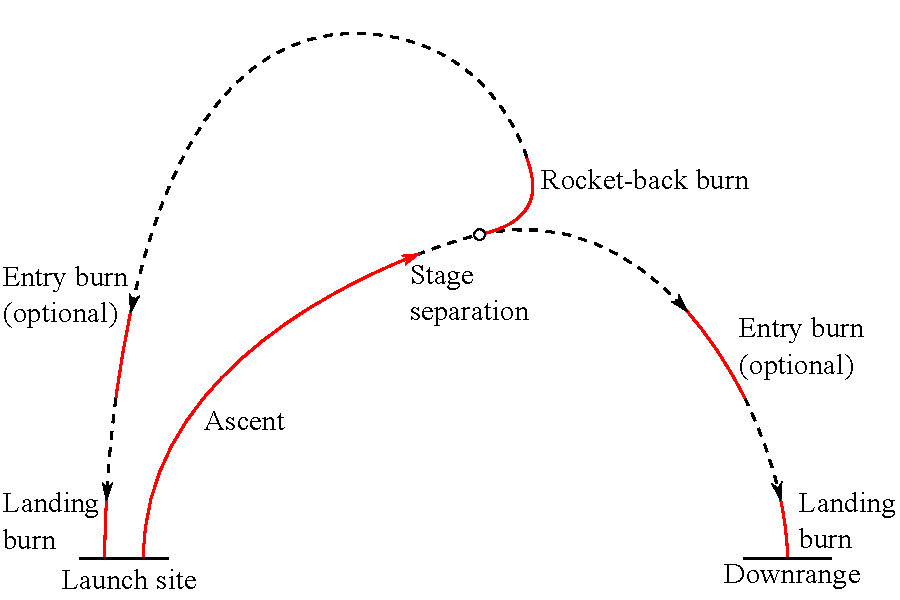
\includegraphics[width=0.5\textwidth]{figures/propulsive_landing}
	\caption{\label{fig:propulsive_landing} Propulsive landing: trajectory options for launch site and downrange recovery. Propulsive portions of the trajectory are shown as red solid lines.}
\end{figure}

The propulsion requirements of these burns is additive, i.e.

\begin{equation}
P = \frac{\Delta v_r}{c_1} = \frac{\Delta v_{rb}}{c_1} + \frac{\Delta v_{e}}{c_1} + \frac{\Delta v_{\mathrm{land}}}{c_1}
\end{equation}

where $\Delta v_{rb}$ is the rocket-back $\Delta v$, $\Delta v_{e}$ is the entry $\Delta v$, and $\Delta v_{\mathrm{land}}$ is the landing $\Delta v$ \footnote{Different values of $c_1$ may be used in each of the terms to account for variations of specific impulse at the different altitudes of the burns.}.



%%% Rocketback %%%
The rocket-back and entry maneuver $\Delta v$s both depend on the magnitude of velocity at stage separation. This will be

\begin{equation}
v_{ss} = - c_1 \ln\left( \epsilon_1' + (1 - \epsilon_1') \pi_1 \right) - \Delta v_{1,loss}
\end{equation}

where $\Delta v_{1,loss}$ is the gravity and drag losses suffered during ascent up to stage separation (typically \SIrange{300}{1000}{\meter\per\second}). Notice that $v_{ss}$ depends on $\epsilon_1'$, which in turn depends on $\Delta v_r$; thus some iteration may be required to find a consistent solution.

Ascent simulations from \cite{Stappert2017} predict that the separation velocity for a variety of recovery strategies will be \SIrange{2100}{3300}{\meter\per\second} (GTO mission, \ce{H2} or hydrocarbon fuels). For Falcon 9, publicly available data from recent launches shows $v_{ss} =$ \SI{1600}{\meter\per\second} (LEO) to \SI{2300}{\meter\per\second} (GTO) \cite{SpaceXWebcast}.

The rocket-back maneuver occurs almost immediately after stage separation. It halts the first stage's downrange motion, and puts the stage onto a nearly ballistic exo-atmospheric trajectory which arcs back toward the launch site. The first stage then enters the sensible atmosphere near the launch site and lands. Because the rocket-back maneuver must halt the horizontal (downrange) component of the first stage velocity, a hard lower limit on $\Delta v_{rb}$ is:

\begin{equation}
\Delta v_{rb} > v_{ss} \cos(\phi_{ss})
\end{equation}

where $\phi_{ss}$ is the flight path angle at stage separation, and might be \SIrange{20}{30}{\degree} \cite{McKinney1986}. The rocket-back maneuver is quite expensive - $\Delta v_{rb}$ will almost certainly be greater than \SI{1300}{\meter\per\second}.

We can learn more about $\Delta v_{rb}$ by considering the near-ballistic return trajectory. After rocket-back shutoff, the stage will have some velocity $v_{rb}$, altitude $z_{rb}$ and flight-path angle $\phi_{rb}$. Assume that the stage must cover a horizontal distance $\Delta x$ back towards the launch site before entering the sensible atmosphere at an altitude $z_e$. The initial velocity magnitude of the ballistic trajectory must be:

\begin{equation}
\label{eq:rocketback_velocity}
v_{rb} = \sqrt{\frac{g_0 \Delta x^2}{\cos[2](\phi_{rb})(z_{rb} - z_{e} + \Delta x \tan(\phi_{rb}))} }
\end{equation}

If the rocket-back burn is performed impulsively, the required $\Delta v$ is:

\begin{equation}
\label{eq:rocketback_dv}
\Delta v_{rb}^2 = v_{rb}^2 + v_{ss}^2 - 2 v_{rb} v_{ss} \cos(\pi - \phi_{rb} - \phi_{ss})
\end{equation}

Under this model, some general trends for $\Delta v_{rb}$ can be observed:
\begin{itemize}
	\item $\Delta v_{rb}$ is reduced for lower $v_{ss}$. If $v_{ss}$ is low, more of the ascent $\Delta v$ must be provided by the second stage. Vehicles with higher $c_2$ (relative to $c_1$) or more mass allocated to the second stage (i.e. higher $y$) will have lower $v_{ss}$ and lower $\Delta v_{rb}$.
	\item $\Delta v_{rb}$ is reduced for steeper ascent trajectories, where $\phi_{ss}$ and $z_{rb}$ are higher and $\Delta x$ is lower.
\end{itemize}

Some estimates of $\Delta v_{rb}$ made with this model are presented in Table \ref{tab:rocketback}. Note that $\Delta v_{rb}$ is very high for GTO launches. Falcon 9 has yet to perform a rocket-back maneuver on a GTO mission, and \cite{Dumont2017} suggests the maneuver may be infeasible even for high-$I_{sp}$ \ce{O2(l)}/\ce{H2(l)} stages.

\begin{table}
	\caption{\label{tab:rocketback} Estimates of rocketback maneuver $\Delta v$ using Eqns. \ref{eq:rocketback_velocity}-\ref{eq:rocketback_dv}. All assume $\phi_{ss}=\ang{25}, \phi_{rb}=\ang{60}$. Range of $\Delta x$, $\Delta z$ for LEO is based on \cite{McKinney1986}}.
	\centering
	\begin{tabular}{l c c}
		Mission & LEO & GTO \\
		\hline
		& $v_{ss} = $\SIrange{1500}{2000}{\meter\per\second} & $v_{ss} = $\SIrange{2100}{3300}{\meter\per\second} \\
		Assumptions & $\Delta x = $ \SIrange{80}{130}{\kilo\meter} & $\Delta x = $ \SIrange{100}{200}{\kilo\meter} \\
		& $\Delta z = $ \SIrange{50}{100}{\kilo\meter} & $\Delta z = $ \SIrange{50}{100}{\kilo\meter} \\
		\hline
		$\Delta v_{rb}$ & \SIrange{1890}{2640}{\meter\per\second} & \SIrange{2500}{4000}{\meter\per\second}
		
	\end{tabular}
\end{table}

The design of the rocket-back trajectory is coupled to the design of the ascent trajectory and possibly to the allocation of mass between the the vehicle stages. An excellent example of optimizing the ascent and rocket-back trajectories can be found in \cite{McKinney1986}. Both the trends predicted from the simple model above are born out in the optimization results: optimal rocket-back vehicles have a steeper ascent trajectory ($\phi_{ss} = $\SIrange{20}{30}{\degree} vs. \ang{10}) and heavier second stages ($y=0.46$ vs $0.20$) than expendable vehicles. A cost-optimal design may also wish to reduce the mass of expended hardware on the second stage, instead of simply maximizing $\pi_*$. Reducing $y$ compared to the designs in \cite{McKinney1986} would tend to increase $\Delta v_{rb}$.

For vehicles with two \ce{O2(l)}/\ce{H2(l)} stages launching to LEO, \cite{McKinney1986} predicts $\Delta v_{rb} =$ \SIrange{2150}{2370}{\meter\per\second}. This agrees with the estimates in Table \ref{tab:rocketback}. McKinney also suggests that a vehicle with a storable propellant booster and a large \ce{O2(l)}/\ce{H2(l)} upper stage would have low $v_{ss}$ and $\Delta v_{rb} \approx$ \SI{1430}{\meter\per\second}.

The entry maneuver $\Delta v$ depends on the heating and dynamic pressure which the vehicle can tolerate. Here designers face a trade-off: to reduce the required $\Delta v_e$ the vehicle could be made more robust (e.g. add heat shields or structural reinforcement), or could be fitted with small wings to fly a shallower, more gentle entry trajectory (e.g. the New Glenn proposal \cite{NewGlenn}). The entry $\Delta v$ for Falcon 9 appears to be $~\SI{800}{\meter\per\second}$ (including $~\SI{200}{\meter\per\second}$ gravity losses; NROL-76 LEO mission after rocket-back) \cite{Dumont2017}\cite{SpaceXWebcast}. If the entry burn specific impulse is \SI{290}{\second}, this contributes 0.28 to $P$. The $\pdv{P}{a}$ trade-off ratio (Eq. \ref{eq:tradeoff_ratio}) suggests that we should be willing devote up to ~30\% of the recovery vehicle dry mass to recovery hardware to forgo this $\Delta v$. For comparison, the mass of wings and thermal protection on the Space Shuttle Orbiter was 17\% of the vehicle mass \cite{Sforza2015}; almost certainly more than would be needed to survive suborbital entry. Thus, it appears payload capacity can be increased by solving the entry problem with additional hardware, not propulsion. Considerations must also be made for how the reentry environment affects component life and refurbishment costs.

%%% Landing %%%
Finally, we will estimate the landing burn $\Delta v_{\mathrm{land}}$. When entering the atmosphere at a steep angle, a low density object such as an almost-empty stage will soon reach a quasi-equilibrium state, falling at its terminal velocity \cite{Wiesel2010}. The landing burn must cancel whatever terminal velocity $v_t$ the stage has when the landing burn begins. The landing burn will also incur some gravity loss. If the landing burn is performed vertically at a constant acceleration $a$, the gravity loss will be $v_t g_0 / a$.

\begin{equation}
\Delta v_{\mathrm{land}} = v_t + \Delta v_{g} = v_t + t_b g_0 = v_t(1 + \frac{g_0}{a})
\end{equation}

The terminal velocity is given by \cite{Wiesel2010}:
\begin{equation}
\label{eq:terminal_velocity}
v_t = \sqrt{\frac{2 m_{\mathrm{ign}} g_0}{C_D(v_t) A \rho_{0}}} \exp\left( \frac{H_\mathrm{ign}}{2H} \right)
\end{equation}

where $m_{\mathrm{ign}}$ is the stage mass at landing burn ignition, $C_D$ is the stage's drag coefficient, $A$ is its frontal area, $\rho_0, H_0$ are the base density and scale height of the atmosphere, and $H_\mathrm{ign}$ is the altitude at landing burn ignition. Unfortunately, $v_t$ may be transonic, so $C_D$ varies significantly with $v_t$. Also, $H_\mathrm{ign} = v_t^2 / (2 a)$.  Thus, Equation \ref{eq:terminal_velocity} must be solved iteratively.

We can make a first guess at $v_t$ using an empirical $C_D(M)$ relation for blunt cylinders from \cite{Hoerner1965}. The resulting terminal velocity is plotted against the stage mass to frontal area ratio in Figure \ref{fig:landing_dv}. The $m_{\mathrm{ign}}/A$ ratio should increase with vehicle size due to cube/square effect. It will likely be \SIrange{1500}{2500}{\kilogram\per\meter\square} for EELV-class stages (data from \cite{wade:atlas, braeunig:delta, wiki:Falcon9FullThrust}), and \SIrange{400}{800}{\kilogram\per\meter\square} for small satellite launchers (data from \cite{electron}). Thus, the landing $\Delta v$ will likely be \SIrange{150}{350}{\meter\per\second}.

Recovery designers have several tools to reduce $\Delta v_{\mathrm{land}}$. High acceleration is favorable for landing burns because it (1) reduces gravity losses and (2) allows the burn to begin deeper in the atmosphere, where the terminal velocity is lower. The terminal velocity can also be decreased by adding deployable drag devices, or by `flying' the stage at a nonzero angle of attack.

Small vehicles have significantly lower landing $\Delta v$ because of their smaller mass/area ratio, however this also causes higher drag losses during ascent.

\begin{figure}[hbt!]
	\centering
	\includegraphics[width=0.7\textwidth]{../landing_dv}
	\label{fig:landing_dv}
	\caption{Variation of landing $\Delta v$ with stage mass / area ratio and landing burn acceleration. TODO draw \& label EELV-class and small sat ranges}
\end{figure}

%%% Summary %%%
In summary, Table \ref{tab:propulsive_strategies} lists the estimated $\Delta v_r$ and $a$ for some variants of the propulsive landing recovery strategy.

\begin{table}
	\caption{\label{tab:propulsive_strategies} Estimates of recovery $\Delta v_r$ and recovery hardware mass $a$ for some variants of the propulsive recovery strategy.}
	\centering
	\begin{tabular}{p{3cm} p{3cm} p{2cm} c c}
		Rocket-back burn? & Entry burn? & Landing burn? & $\Delta v_r$ & $a$ \\
		\hline
		Yes, assume launch to LEO & Yes & Yes & \SIrange{2700}{3800}{\meter\per\second} & \SIrange{0.05}{0.07}{}\\
		No - Downrange landing & Yes & Yes & \SIrange{800}{1150}{\meter\per\second} & \SIrange{0.05}{0.07}{} \\
		No - Downrange landing & No - extra aero/TPS hardware & Yes & \SIrange{150}{350}{\meter\per\second} & \SIrange{0.05}{0.22}{}\\
		\hline
	\end{tabular}
\end{table}


\subsubsection{Winged, horizontal landing}
In horizontal landing strategies, the recovery vehicle is equipped with wings and landing gear, and lands horizontally like an airplane. The recovery can take place downrange, or the recovery vehicle can fly back to the launch site, although the latter probably requires the vehicle to be equipped with air-breathing engines as well. Horizontal landing strategies have been proposed for full and partial recovery. The main performance penalty for horizontal landing is due to the additional inert mass required compared to an expendable system.

The recovery hardware mass includes wings, control surfaces, thermal protection, and possibly an air-breathing propulsion system. The mass of these components are best estimated by analogies to other winged vehicles. The Space Shuttle Orbiter will represent the extreme of fast, small-winged aircraft, while the C-141 will represent the extreme of slow, large-winged aircraft. Table \ref{tab:winged_strategies} lists the estimated contributions to the recovery hardware mass. For a glider recovery vehicle, we should expect $a = \SIrange{0.18}{0.37}{}$. Including air-breathing propulsion for powered flyback will probably increase $a$ to \SIrange{0.28}{0.52}{}. In the NASA LFBB proposal, $a=0.52$ \footnote{assuming the baseline hardware to be recovered makes up $E_1=0.08$ of the gross liftoff mass, and using mass estimates from \cite{Healy1998}}.

\begin{table}
	\caption{\label{tab:winged_strategies} Estimates of recovery hardware mass $a$ for horizontal landing recovery strategies. Data from \cite{Sforza2015}.}
	\centering
	\begin{tabular}{l c}
		Vehicle system/component  & Fraction of recov. vehicle dry mass ($a$) \\
		\hline
		Wing                      & \SIrange{0.061}{0.16}{} \\
		Tail                      & \SIrange{0.012}{0.027}{}\\
		Landing gear              & 0.05 \\
		Surface controls          & \SIrange{0.01}{0.02}{} \\
		Thermal protection        & \SIrange{0.05}{0.11}{} \\
		Propulsion, air breathing & \SIrange{0.1}{0.15}{} \\
		\hline
		Glider total         & \SIrange{0.18}{0.37}{} \\
		Powered flyback total        & \SIrange{0.28}{0.52}{} \\
		\hline
	\end{tabular}
\end{table}


\begin{figure}[hbt!]
	\centering
	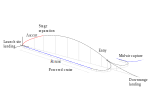
\includegraphics[width=0.7\textwidth]{figures/flyback_trajectory}
	\caption{\label{fig:flyback_trajectory} Horizontal landing: trajectory options for launch site and downrange recovery. Portions of the trajectory flown under rocket propulsion are shown as red solid lines; air-breathing propulsion is indicated with blue.}
\end{figure}

Next, the landing location must be considered, as it may drive the need for additional propulsion during the recovery flight. The recovery vehicle may be able to return to the launch site by gliding, but this is only feasible for very low stage separation velocities (<\SI{1000}{\meter\per\second} \cite{Hellman2005} \cite{Healy1998}). Otherwise, the recovery vehicle will either need to land downrange, or have propulsion during the recovery flight. If the risk of a launch over land can be tolerated, the recovery vehicle can simply land at a downrange airport. However, safety concerns will typically require downrange recovery to occur in the ocean. There are several options for recovering a horizontal-landing vehicle over the ocean.
 
 \begin{itemize}
 	\item \emph{Landing directly in the ocean} - This risks damage to the stage by salt water intrusion and wave action, and will probably lead to high recovery and refurbishment costs.
 	\item \emph{Landing on a ship} - The practicality of this option depends on the size and stall speed of the vehicle. Aircraft with similar mass to an empty EELV booster (e.g. A-3 Skywarrior, \SI{37}{\mega\gram} \cite{DouglasA3}) have been operated from ships. However, a vehicle with small wings for reentry would likely have a high touchdown speed (e.g. \SI{100}{\meter\per\second} for the Orbiter \cite{ShuttleLanding} vs. \SI{65}{\meter\per\second} for typical carrier landings \cite{Shen2013}), increasing the difficulty of arresting the vehicle on a ship's deck. The vehicle may also need heavier landing gear and structural reinforcement to interface with the arrest system. On the whole, this approach seems plausible only for small rockets or partial recovery strategies.
 	\item \emph{Mid-air capture} - The recovery vehicle is hooked by a powered aircraft in mid-air, and is then towed back to near the launch facility. The recovery vehicle then disconnects the tow line and lands as a glider (see \cite{Stappert2017}).
 \end{itemize}

If none of the downrange recovery recovery options are acceptable, the recovery vehicle must also carry an air-breathing propulsion system to power the return flight, incurring a significant mass and complexity penalty.
The C-141 example suggests that air-breathing engines will add about 12\% to the vehicle mass. A recovery vehicle may be able to use smaller engines, as it only needs enough thrust for cruise, not takeoff. However, the recovery vehicle will also need larger, perhaps moving, nacelles to protect the air-breathing engines during ascent and entry \cite{Healy1998}, which would add extra mass.

Additional fuel must also be carried for the air-breathing engine. The mass of fuel for the air-breathing engine is calculated from the Berguet range equation (Eq. \ref{eq:berguet_p}). We should expect the cruise range $R_{\mathrm{cruise}}$ to be \SIrange{370}{570}{\kilo\meter} \cite{Healy1998, Hellman2005} and $v_{\mathrm{cruise}} = \SI{150}{\meter\per\second}$ \cite{Healy1998}. The engine efficiency for a low-bypass turbofan should be about $I_{sp}^{\mathrm{a.b.}} = \SI{3600}{\second}$ \cite{Hellman2005}. The cruise $L/D$ would be around 4 for a vehicle with small delta wings \footnote{this could be increased by using high aspect ratio folding wings, as mentioned in \cite{Healy1998} and some Soviet proposals for reusable Energia II boosters. The folding mechanism would incur and additional mass penalty.}. Under these assumptions, $P$ will be between $0.17$ and $0.26$. In the NASA LFBB proposal, $P=0.20$ \cite{Healy1998}.


\subsubsection{Parachute recovery}
In parachute recovery, the 

SRB parachutes were 3.5\% of booster dry mass \cite{Wolf1996}. Guessing TPS another 2\% (\SI{500}{\kilogram\per\meter\cubed}, 0.25 inch thick)???

Liquid stage parachute recovery attempts have failed, breakup during reentry \cite{
Spencer2011}.
TODO



TODO propulsive strategy gives more operational flexibility between recover and expend modes. Easy to reallocate recovery propellant to ascent to use the vehicle in a higher-payload expendable mode.  Harder to remove wings.



\section{Cost Model}
Next, we attempt to quantify the cost savings from reusing the first stage. The cost savings are quantified by the cost factor $r_c$, which is the ratio of the average cost of one flight of a reusable first stage to the average cost of an expendable first stage. For $r_c < 1$, the reusable system has lower recurring costs. Write $r_c$ in terms of some of the cost elements identified in \cite{Sforza2015}:

\begin{equation}
\label{eq:cost_elements}
r_c = \frac{\frac{C_{pr}}{n} + C_{pn} + C_f + C_{ro}}{C_{pe}}
\end{equation}

where $n$ is the average lifetime number of flights for a reusable first stage. The cost elements of the reusable first stage are: $C_{pr}$, the production cost of the reusable components; $C_{pn}$, the production cost of the new (non-reusable) components; $C_f$, the refurbishment cost; and $C_{ro}$, the recovery operations cost. The expendable stage production cost is $C_{pe}$. Note that this cost model does not capture development costs. Also, $r_c$ only includes those costs directly relevant to the first stage, and excludes other factors which contribute to the launch service cost (upper stage, facilities, and insurance, etc.).

Actual costs vary with booster size scale, are difficult to estimate for new vehicle proposals \cite{Sforza2015}, and are often not publicly available. Instead, it is more helpful to write the cost factor in terms of dimensionless ratios which can be more readily estimated. I define the following ratios:
\begin{itemize}
	\item The recovered cost ratio, $z$, which is the ratio of the cost of the recovered hardware to the total production cost of the recoverable stage
    \begin{equation}
    z = \frac{C_{pr}}{C_{pr} + C_{pn}}
    \end{equation}
    By definition, $z \in [0, 1]$. For full-recovery strategies, $z=1$. For strategies which recover only the engines and other high-value components, $z \approx 0.5$ \cite{Ragab2015} (TODO more general engine cost as fraction of stage cost. I think Atlas V has a unusually expensive engine).
    
    \item The recovery and refurbishment cost ratio, $q$, which is the cost of recovery and refurbishment divided by production cost of the reusable hardware.
    \begin{equation}
    q = \frac{C_{f} + C_{ro}}{C_{pr}}
    \end{equation}
    By definition, $q > 0$. Inefficient recovery strategies can have $q > 1$, in which case recovery cannot lead to cost savings and is probably not worthwhile. In some extreme proposals, the only recovery/refurbishment operation would be to reload the stage with propellant \cite{Musk2017}. In this case, propellant costs give a lower limit of $q \approx 0.01$ for hydrocarbon/oxygen stages \cite{Ragab2015}. A more moderate estimate from \cite{Sforza2015} gives $q \approx 0.25$ (15\% for refurbishment and another 10\% for recovery operations). It should be expected that downrange recovery strategies will incur higher $q$ than launch site recovery, due to the added cost of shipping back the stage. Further, landing directly in the ocean likely increases $q$ due to salt water damage. Practical data on first stage recovery and refurbishment costs is limited. In the Space Shuttle program, SRB recovery and refurbishment almost exceeded production costs ($q \approx 1$) [TODO citation needed]. Refurbishment cost data for Falcon 9 is not publicly available, but SpaceX leadership has stated that the refurbishment cost of the first Falcon 9 booster to be re-used was ``substantially less than half'' of the production cost ($q<0.5$) \cite{Foust2017}.
   
    \item The production cost ratio, $b$, which is the ratio of production costs for reusable and expendable stages.
    \begin{equation}
    b = \frac{C_{pr} + C_{pn}}{C_{pe}}
    \end{equation}
    We should expect that, all other factors being equal, reusable stages will be more expensive to produce, so $b>1$. Several factors increase the cost of reusable stages:
    \begin{itemize}
    	\item Extra hardware - Recovery devices (which are not required on an expendable version) add to the production cost. The magnitude of this effect is difficult to estimate in a general manner.
    	\item More durable hardware - More expensive materials or designs may be employed to extend component life. The magnitude of this effect may increase weakly with $n$, but is  difficult to estimate in a general manner.
    	\item Lower production rate - If a reusable and expendable fleet are to provide the same total number of launches \footnote{This may not be a good assumption - if a fleet has significantly lower launch costs, it may be able to capture a larger share of the launch market or increase the volume of the launch market}, the expendable fleet will require $n$ times more first stages. Due to experience curve effects, the average cost of producing a stage is expected to decline as the production volume increases. The average reusable stage production cost would therefore be higher, even if the first-unit costs are identical. If the experience curve is described by a power law with learning rate $s$, then
    	\begin{equation}
    	b = \frac{C_{pr}' n^{-\log_2(s)} + C_{pn}'}{C_{pe}'}
    	\end{equation}
    	where primes denote first-unit costs (as opposed to average costs).
    \end{itemize}
\end{itemize}

Using these factors, Equation \ref{eq:cost_elements} can be re-written as

\begin{equation}
\label{eq:r_c_dimensionless}
r_c = z b \left( \frac{1}{n} + \frac{1 - z}{z} + q \right)
\end{equation}

There is substantial uncertainty and project-to-project variation in the cost ratios $b$ and $q$, so we should not expect to predict a single, general value for $r_c$. However, we can establish some plausible bounds on $r_c$ for the full and partial reuse cases. In the limit of a ``perfectly reusable'' stage ($n\rightarrow\infty, b=1, q=0$), Equation \ref{eq:r_c_dimensionless} reduces to $r_c = 1 - z$. This puts a hard lower limit on the cost factor for partial reuse strategies:

\begin{equation}
\label{eq:r_c_low_limit}
r_c > 1 - z
\end{equation}

The cost model is further explored in Figure \ref{fig:cost_model}, which shows contours of $r_c$ over a plausible range of $q$ and $b$. Each subplot shows an different scenario for the recovered cost ratio $z$ and the component life $n$. Several interesting factors are apparent. First, partial recovery strategies ($z=0.5$, right column of plots) are more sensitive to changes in the production cost ratio $b$, and are impractical for $b>2$ even with long life and low refurbishment costs. Second, full recovery strategies can offer large 1st stage cost savings (low $r_c$) if the refurbishment costs are kept low and the stages have long lifetimes, even if production costs for reusable stages are relatively high. In a full-recovery strategy, it is likely worthwhile to make design changes which can streamline refurbishment and increase life, even if they increase the production cost.

\begin{figure}[hbt!]
	\centering
	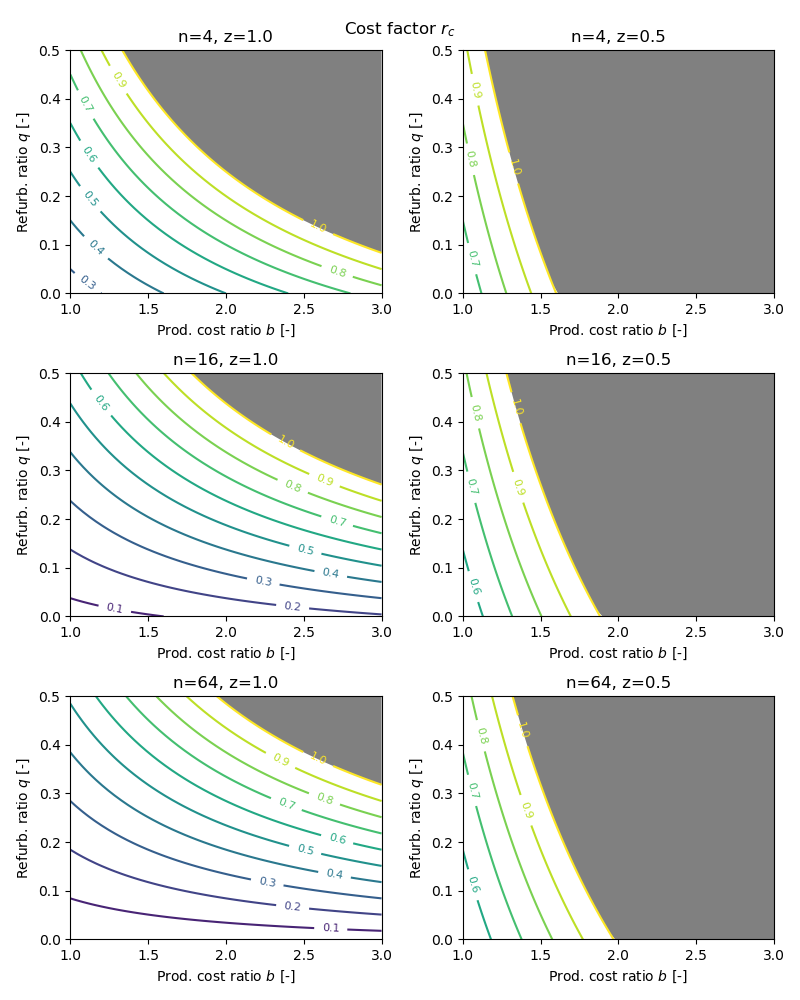
\includegraphics[width=1\textwidth]{../cost_model}
	\label{fig:cost_model}
	\caption{First stage re-use cost factor $r_c$ as a function of the recovery and refurbishment cost ratio $q$ and the production cost ratio $b$. Impractical regimes where re-use would not reduce cost ($r_c>1$) are shaded grey. The plots in the left column correspond to full recovery strategies ($z=1$), and the right to partial recovery ($z=0.5$). The top row corresponds to a conservative reusable component life ($n=4$ flights), the middle to a moderate life ($n=16$) and the bottom to an optimistic life ($n=64$).}
\end{figure}

To facilitate later comparisons of full vs partial recovery strategies, I compute their cost ratios in two scenarios: one making optimistic assumptions about the other variables in the reuse cost model, and one making more moderate assumptions. Table \ref{tab:cost_scenarios} shows that we can reasonably expect the cost factor to be between $0.05$ and $0.52$ for full recovery, and $0.78$ or more for partial recovery. The moderate-assumption case agrees with other assessments that a fully reusable first stage can reduce launch costs "by a factor of 2 to 3" \cite{Hampsten2010}.

\begin{table}
\caption{\label{tab:cost_scenarios} Cost factor $r_c$ in hypothetical reuse scenarios}
\centering
\begin{tabular}{lcc}
\hline
& Optimistic & Moderate \\
& $q=0.02, b=1.5, n=64$ & $q=0.20, b=2.0, n=16$ \\
\hline
Full recovery $z=1$ & 0.05 & 0.53 \\
Partial recovery $z=0.5$ & 0.78 & 1.3 \\
\hline
\end{tabular}
\end{table}


\section{Cost \& Performance Tradeoffs/Comparison}
TODO
The trade a launch operator is willing to make depends on many complicated, context specific factors (cost structure, payload discretization, etc.). Therefore, it is not possible to specify a single strategy as being `best'. Rather, this section seeks to identify the set of Pareto-optimal strategies, each of which offers the greatest payload for a certain level of cost reduction.

Pareto set of best strategies.


\bibliography{first_stage_recovery}

\end{document}